\hypertarget{predicate_8cpp}{}\section{src/proposition/predicate.cpp File Reference}
\label{predicate_8cpp}\index{src/proposition/predicate.\+cpp@{src/proposition/predicate.\+cpp}}
{\ttfamily \#include $<$algorithm$>$}\newline
{\ttfamily \#include \char`\"{}predicate.\+h\char`\"{}}\newline
{\ttfamily \#include \char`\"{}../notation/and.\+h\char`\"{}}\newline
{\ttfamily \#include \char`\"{}../notation/biimplicate.\+h\char`\"{}}\newline
{\ttfamily \#include \char`\"{}../notation/exists.\+h\char`\"{}}\newline
{\ttfamily \#include \char`\"{}../notation/forall.\+h\char`\"{}}\newline
{\ttfamily \#include \char`\"{}../notation/implicate.\+h\char`\"{}}\newline
{\ttfamily \#include \char`\"{}../notation/nand.\+h\char`\"{}}\newline
{\ttfamily \#include \char`\"{}../notation/negate.\+h\char`\"{}}\newline
{\ttfamily \#include \char`\"{}../notation/or.\+h\char`\"{}}\newline
{\ttfamily \#include \char`\"{}../notation/value.\+h\char`\"{}}\newline
{\ttfamily \#include \char`\"{}../notation/variable.\+h\char`\"{}}\newline
{\ttfamily \#include \char`\"{}../notation/statement.\+h\char`\"{}}\newline
Include dependency graph for predicate.\+cpp\+:\nopagebreak
\begin{figure}[H]
\begin{center}
\leavevmode
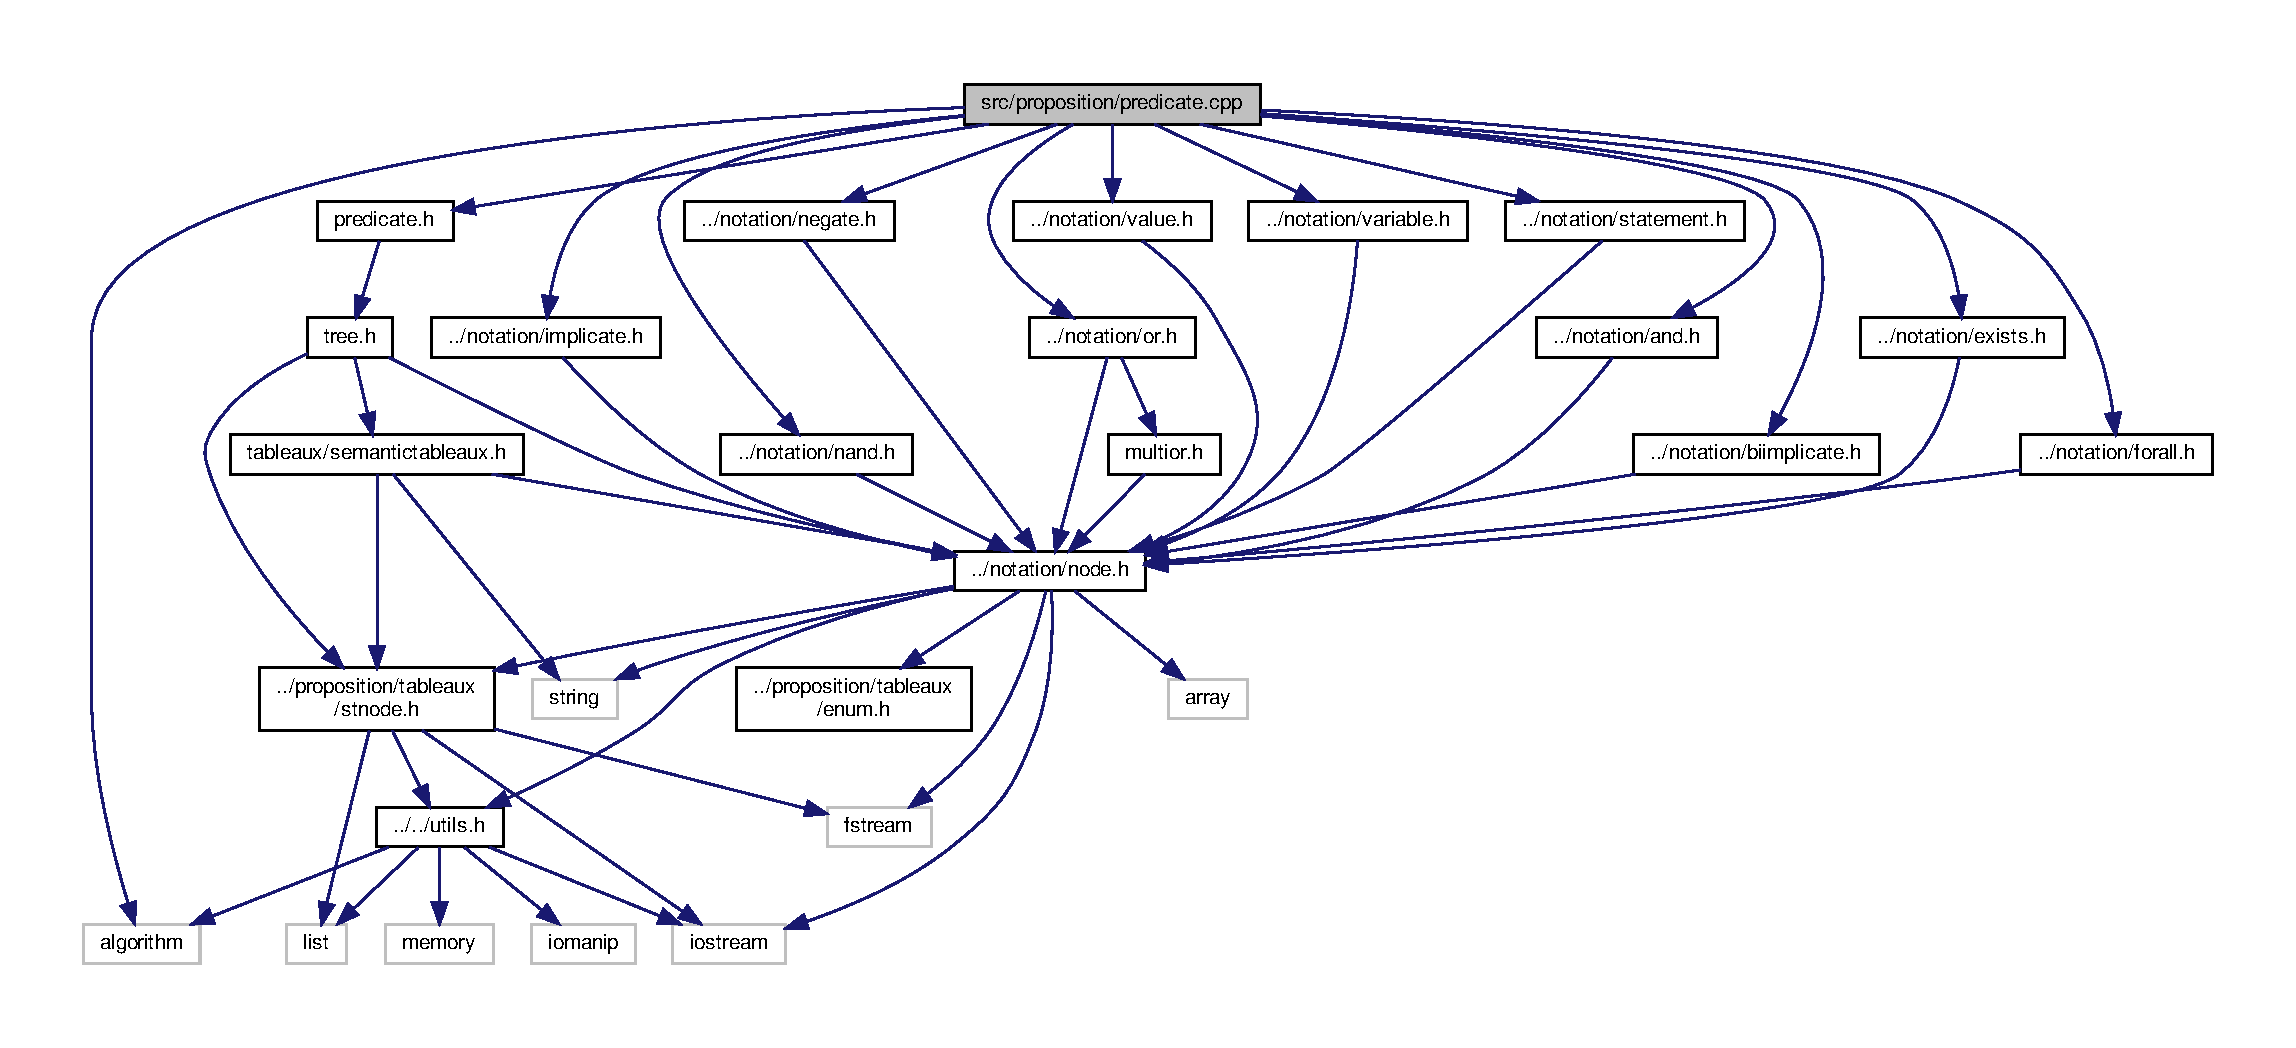
\includegraphics[width=350pt]{d4/d54/predicate_8cpp__incl}
\end{center}
\end{figure}
